\section{Trigonometric functions}

Spivak covers variations of trigonometric functions as he goes through
the book. I initially found it distracting-- it's hard enough to
understand $\epsilon-\delta$ limits; it's harder still if you're also trying to
learn trig as you go. But trig is important, and sooner or later it's
time to understand it. That time is now. Here I introduce the basics
of trigonometric functions, and then cover everything trig-related
from Spivak's early chapters that I ignored in these notes until now.

\subsection{Definitions}

Let $P$ be a point on a unit circle $x^2+y^2=1$. Let $\theta$ be the length
of the arc from $(1,0)$ to $P$, measured counterclockwise along the
circle. Then the coordinates of $P$ are
$(\cos\theta,\sin\theta)$.\footnote{The order is easy to remember-- it's
  alphabetical.}

\begin{figure}[htbp]
  \centering
  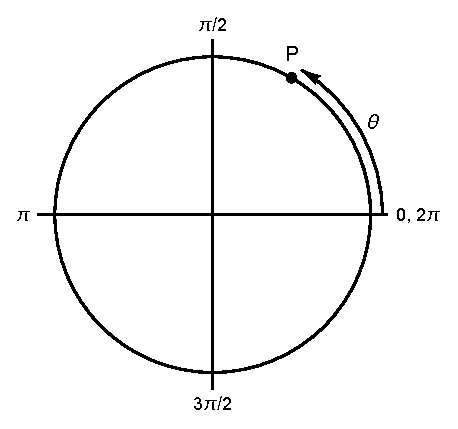
\includegraphics[width=0.5\textwidth]{eps/prereqs/trigtldr.eps}
\end{figure}

The measure of angles by the length of the arc is in units called
\textit{radians}. Recall the circumference of a circle is $C=2\pi r$,
and so the circumference of a unit circle is $2\pi$. Thus $\pi$ represents
a $180^\circ$ angle. Some common angles in radians are
$2\pi, \pi,\frac{\pi}{2}, \frac{\pi}{3}, \frac{\pi}{4}, \frac{\pi}{6}$, and
$\frac{3\pi}{2}$. To convert these to degrees simply replace $\pi$ with
$180$, and compute the fraction.

\vs

It should be self-evident that adding $2\pi$ to an angle results in the
angle itself; and that adding $\frac{\pi}{2}$ to an angle shifts it by
$90^{\circ}$. Further:
\[(\cos 0,\sin 0)=(1,0)\ \ \ \ \ \text{and}\ \ \ \ \ (\cos \frac{\pi}{2},\sin \frac{\pi}{2})=(0,1)\]

\clearpage
\subsubsection*{Plotting}
It is not too difficult to plot trigonometric functions. Consider some
properties of cosine we've already seen (or can easily deduce):
$\cos 0=1$, $\cos \frac{\pi}{2}=0$, $\cos \pi=-1$. We've also seen that
$\cos{(x+2\pi)}=\cos x$. The $x$-axis below covers $[-3\pi, 3\pi]$ (i.e. a
total length of $6\pi$). Since cosine repeats every $2\pi$, we should
expect the graph to repeat thrice. And this is exactly what we see.
\begin{figure}[htbp]
  \centering
  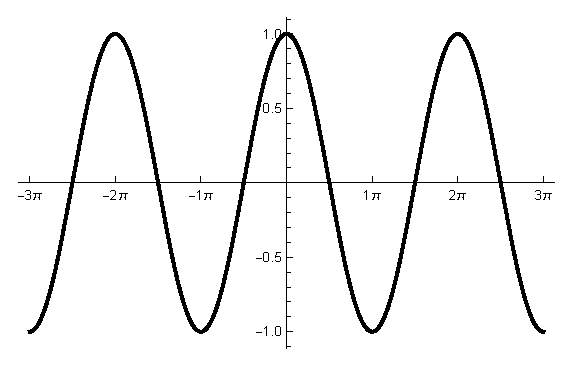
\includegraphics[width=.75\textwidth]{eps/prereqs/cosine.eps}
\end{figure}

We can easily increase the frequency by plotting $y=\cos cx$. Here we
double the frequency with $c=2$:
\begin{figure}[htbp]
  \centering
  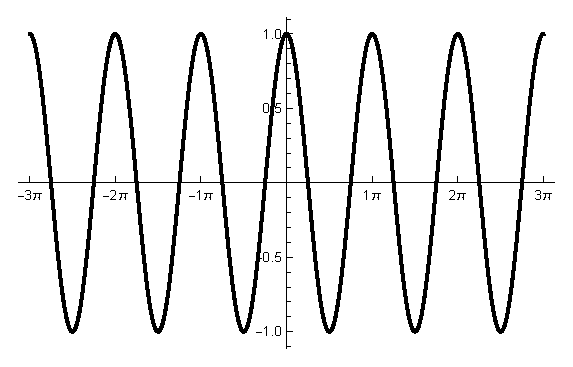
\includegraphics[width=.75\textwidth]{eps/prereqs/cosine2x.eps}
\end{figure}

\clearpage
\subsection{Limits}

\textbf{Claim 1a:} Let $f(x)=x\sin \frac{1}{x}$. Then
$\lim_{x\to0}f(x)=0$.

\textbf{Proof.} Let $\epsilon>0$ be given. We must show
$0<|x-0|<\delta$ implies $|f(x)-0|<\epsilon$. This is easy if you recall
the co-domain of $\sin$ is $[-1,1]$. This implies:
\[\left|x\sin \frac{1}{x}\right|\leq |x|\]

Thus fixing $|x|<\epsilon$ implies
$\left|x\sin \frac{1}{x}\right|<\epsilon$ as desired.



\vs---\vs

\textbf{Claim 1b:} Let $f(x)=x^2\sin \frac{1}{x}$. Then
$\lim_{x\to0}f(x)=0$.

\textbf{Proof.} By the same reasoning as above,
$\left|x^2\sin \frac{1}{x}\right|\leq x^2$. Thus fixing $|x|<\sqrt{\epsilon}$
implies $\left|x^2\sin \frac{1}{x}\right|<\epsilon$ as desired.

\vs---\vs

\textbf{Claim 1c:} Let $f(x)=\sqrt{|x|}\sin \frac{1}{x}$. Then
$\lim_{x\to0}f(x)=0$.

\textbf{Proof.} By the same reasoning as above,
$\left|\sqrt{|x|}\sin \frac{1}{x}\right|\leq \sqrt{|x|}$. Thus fixing
$|x|<\epsilon^2$ implies
$\left|\sqrt{|x|}\sin \frac{1}{x}\right|\leq \epsilon$ as desired.


\vs---\vs

\textbf{Claim 2:} $\lim_{x\to0}\sin \frac{1}{x}$ does not exist.

\textbf{Proof.}

\vs---\vs

\textbf{Claim 3:} $\lim_{x\to\infty}\sin \frac{1}{x}=0$.

\textbf{Proof.}

\subsection{Continuity}

\textbf{Claim 1:} $f(x)=\sin \frac{1}{x}$, $g(x)=x\sin \frac{1}{x}$ are not continuous at $0$.

\textbf{Proof.}

\vs---\vs

\textbf{Claim 2:} Let
\[G(x)=\begin{cases}
  x\sin \frac{1}{x},&x\neq0\\
  0,&x=0
\end{cases}\]
Then $G$ is continuous at $0$.

\vs

\textbf{Proof.}

\vs---\vs

\textbf{Claim 3:} Let
\[F(x)=\begin{cases}
  \sin \frac{1}{x},&x\neq0\\
  a,&x=0
\end{cases}\]
Then $F$ is \textit{not} continuous at $0$, for any choice of $a$.

\vs

\textbf{Proof.}

\vs---\vs

\textbf{Claim 4:} Let
\[f(x)=\begin{cases}
  x\sin \frac{1}{x},&x\neq0\\
  0,&x=0
\end{cases}\]
Then $f$ is continuous at $a$ for $a\neq 0$.

\vs

\textbf{Proof.}


\subsection{Derivatives}

\textbf{Claim 1:} Let
\[f(x)=\begin{cases}
  x\sin \frac{1}{x},&x\neq0\\
  0,&x=0
\end{cases}\]
Then $f$ is not differentiable at $0$.

\vs

\textbf{Proof.}

\vs---\vs

\textbf{Claim 2:} Let
\[g(x)=\begin{cases}
  x^2\sin \frac{1}{x},&x\neq0\\
  0,&x=0
\end{cases}\]
Then $g$ is differentiable at $0$.

\vs

\textbf{Proof.}

\subsection{Differentiation}

\textbf{Claim 1:} $g'$ is not differentiable at $0$.

\textbf{Proof.}

\vs---\vs

\textbf{Claim 2:} Let
\[f(x)=\begin{cases}
  x^3\sin \frac{1}{x},&x\neq0\\
  0,&x=0
\end{cases}\]
Then $f'$ is not differentiable at $0$.

\vs

\textbf{Proof.}

\vs---\vs

\textbf{Claim 3:} Let
\[f(x)=\begin{cases}
  x^4\sin \frac{1}{x},&x\neq0\\
  0,&x=0
\end{cases}\]
Then $f''$ is not differentiable at $0$.

\vs

\textbf{Proof.}

\vs

\textbf{TODO more stuff on pp 178}

%%% Local Variables:
%%% TeX-master: "notes"
%%% End:
